%\documentclass{article}

%\usepackage[utf8]{inputenc}
% \usepackage{amsmath}
%\usepackage{amsthm}
%\usepackage{amssymb}
%\usepackage{float}
%\usepackage{graphicx}
%\usepackage[a4paper, total={6in, 10in}]{geometry}
%\usepackage{array}



% -----------------------------------------------------------------------------
\documentclass[a4paper]{artikel3}
% -----------------------------------------------------------------------------
\paperheight = 29.70 cm  \paperwidth = 21.0 cm  \hoffset        = 0.46 cm
\headheight  =  0.81 cm  \textwidth  = 15.0 cm  \evensidemargin = 0.00 cm
\headsep     =  0.81 cm	 \textheight = 9.00 in  \oddsidemargin  = 0.00 cm					
% -----------------------------------------------------------------------------
\usepackage{enumerate}
\usepackage{amsfonts}
\usepackage{amsmath}
\usepackage{url}
\usepackage{graphicx}
\usepackage{float}
\usepackage[font=small,labelfont=bf]{caption}
\usepackage{setspace}
\usepackage{booktabs}
\usepackage{threeparttable}
\usepackage[
		    colorlinks=true, 
		    urlcolor=blue, 
		    linkcolor=blue, 
		    citecolor=blue, 
		    pdfstartview=FitH]{hyperref}
\usepackage{array}
\usepackage[svgnames]{xcolor}
\usepackage[tikz]{bclogo}
\usepackage{listings}
\usepackage{lstbayes}
\bibliographystyle{elsarticle-num}
\usepackage{xcolor}
\usepackage{subfigure} 
\usepackage{geometry}
\definecolor{codegreen}{rgb}{0,0.6,0}
\definecolor{codegray}{rgb}{0.5,0.5,0.5}
\definecolor{codepurple}{rgb}{0.58,0,0.82}
\definecolor{backcolour}{rgb}{0.95,0.95,0.92}

\lstdefinestyle{mystyle}{
    language=TeX,
    backgroundcolor=\color{white},   
    commentstyle=\color{codegreen},
    keywordstyle=\color{magenta},
    numberstyle=\tiny\color{codegray},
    stringstyle=\color{codepurple},
    basicstyle=\ttfamily\footnotesize,
    breakatwhitespace=false,         
    breaklines=true,                 
    captionpos=b,                    
    keepspaces=true,                 
    numbers=left,                    
    numbersep=5pt,                  
    showspaces=false,                
    showstringspaces=false,
    showtabs=false,
    deletekeywords=[2]{hash,beta},
    tabsize=2
}

\lstset{style=mystyle}
\geometry{a4paper,left=1cm,right=2cm,top=2cm,bottom=2cm}
% -----------------------------------------------------------------------------
\newtheorem{thm}{Theorem}
\newtheorem{cor}[thm]{Corollary}
\newtheorem{lem}{Lemma}
\newtheorem{prop}{Proposition}
\newtheorem{definition}[thm]{Definition}
\newtheorem{rem}[thm]{Remark}
\newtheorem{exm}[thm]{Example}
% -----------------------------------------------------------------------------
\newcommand{\norm}[1]{\left\Vert#1\right\Vert}
\newcommand{\abs}[1]{\left\vert#1\right\vert}
\newcommand{\set}[1]{\left\{#1\right\}}
\newcommand{\Real}{\mathbb R}
\newcommand{\eps}{\varepsilon}
\newcommand{\To}{\longrightarrow}
\newcommand{\mb}[1]{\mathbf{#1}}
\newcommand{\gb}[1]{\text{\boldmath$#1$}}
\newcommand{\ov}[1]{\overline{#1}}
\newcommand{\mml}{\{}
\newcommand{\mmr}{\}}
\newcommand{\lh}[1]{\widehat{#1}}
\newcommand{\pname}[1]{\textsc{#1}}
\newcommand{\lc}[1]{\mathscr{#1}}
\newcommand{\lcs}[1]{\ov{\mathscr{#1}}}
\newcommand{\lco}[1]{\overline{\mathscr{#1}}}
\newcommand{\lch}[1]{\widehat{\mathscr{#1}}}
\newcommand{\spi}{\ell}
\newcommand{\zf}[1]{z(#1)}
\newcommand{\R}{\mathbb{R}}
% -----------------------------------------------------------------------------
\allowdisplaybreaks
\onehalfspacing
% -----------------------------------------------------------------------------
\begin{document}


% Title page
\begin{center}
{\Large \onehalfspacing \bf Predict the prabability of occurence of different kinds of fishes in south-western Ohio}
\end{center}
\vspace{10pt}
\begin{center}
\large Authors: Zhiqiang Liao$^1$, Zhenkun Li$^2$, Mohamed Nazaal Ibrahim$^3$\\
\end{center}

\begin{flushleft}
$^1$ Department of Information and Service Management, School of Business, Aalto University. \\
$^2$ Department of Computer Science, School of Science, Aalto University. \\
$^3$ Department of Civil Engineering, School of Engineering, Aalto University. 
\end{flushleft}
%\date{\today}

%\maketitle
% \begin{bclogo}[logo=\bcattention, couleurBarre=red, noborder=true, 
%                couleur=LightSalmon]{Important links}
%     \begin{itemize}
%         \item \href{https://avehtari.github.io/BDA_course_Aalto/project_work/rubric.pdf}{Project rubric}
%         \item \href{https://raw.githubusercontent.com/avehtari/BDA_course_Aalto/gh-pages/project_work/slides_project_work.pdf}{Project work details slides}
        
%     \end{itemize}
% \end{bclogo}

\normalsize
\section{Introduction}
Ecological risk assessments (ERA) are a critical component of environmental decision making, as the ability to make sound risk management decisions rests heavily on the information they provide \cite{barnthouse2007population}. In this project, we use a logistic regression model to predict the presence-absence state of environmental stressors (e.g., toxic chemicals), which has been proven highly related to fish community health \cite{miltner2010method}. Compared to the traditional ERA methods, our project provides an alternative and inexpensive way for decision-makers to environmental risk management.


\subsection{Motivation}
The traditional ERA process usually requires specialized models, data, and expertise, which can be cost and time-intensive. Alternatively, data-driven prediction models that use Geographic Information Systems (GIS) data are often attractive to practitioners and researchers because they offer a cost-effective way of quickly detecting areas of potential risk across broad regions; and can inform future, more targeted research activities \cite{martin2018empirically}. In this project, we use the recently published StreamCat database, which includes a comprehensive list of segment and watershed-scale metrics for use with the NHDPlus dataset within the conterminous United States \cite{hill2016stream}. 

This project follows the research paper of Martin et al. \cite{martin2018empirically}. In this paper, the authors applied a Bayesian separate model with a latent variable. The main idea of this study is to analyze the correlation between stressors (e.g., toxic chemicals) and ecological receptors (e.g., fishes). Although we use the same dataset as the original paper, we consider a different task which is to predict the presence-absence state of the environmental stressors. To do so, we choose total phosphorus (TP) as a response variable and three measures derived from GIS database sources as predictors. This question is also interesting given the real-time available GIS data. 

In this project, we use two Bayesian models to predict the environmental risk of the watershed. We believe the proposed models would help decision-makers who are responsible for environmental risk management.


\subsection{Problem}
In a recent study of Ohio streams, Miltner (2010) examined the effects of TP on fishes using statewide bioassessment data and suggested a seasonal average for TP at 0.1 mg/L as a feasible management target for improving fish community health and to aid future abatement and prevention of eutrophication in Ohio streams (b1300 km2 in drainage area; Miltner, 2010).

The research team from the Ohio Environmental Protection Agency measured 83 bioassessment sites collected over the summer of 2012. In the dataset, they collected 26 stressors (i.e., TP), in which we choose TP as response variable. We used this management criterion to examine the effects of excess nutrients on potentially sensitive fishes and their distributions. Thus, TP concentration data (mg/L) for each bioassessment site were converted to binary variables depending on whether values were below or above 0.1 mg/L. As the notation of the following section, our outcome variable is
\begin{equation*}
y_n =
    \begin{cases}
        1 & \text{if the site $n$ is environmental risk for fishes}\\
        0 & \text{if the site $n$ is environmental health for fishes}
    \end{cases}
\end{equation*}

\subsection{Main modeling idea}


In the original paper \cite{martin2018empirically}, the authors chose informative priors for all 27 responses (corresponding to records of presence-absence for fishes). The proposed separate Bayesian method cannot sufficiently fit a model including different types of responses, though the authors suggested that they could have chosen different types of priors (e.g., informative, weakly informative) for each parameter and response combination in order to fit a model including all 77 responses.

First, we propose a hierarchical model to handle this problem in this project.

\subsection{Illustrative figure}

\section{Description of the data and the analysis problem}
\subsection{Descriptive statistics}
The response data, Y, comprised empirical data from 28 responses measured across 83 sites in the EFLMR watershed; with 27 of the responses corresponding to records of presence-absence for fishes and 1 response corresponding to records of TP exceeding the management threshold of 0.1 mg/L. The input data, X, included three predictors: drainage area, crop cover, and septic tank counts. All predictor variables were standardized prior to input into the models by subtracting the mean and dividing by 2 standard deviations.

In Table \ref{tab: data}, we summarize the descriptive statistics of input data from the NHDPlus hydrologic spatial dataset \cite{moore2019user} and response data from EFLMR watershed dataset by the Ohio Environmental Protection Agency's (OEPA) Statewide Biological and Water Quality Monitoring and Assessment Program. Note that we omit the data of 27 fishes because of the limitation of space. The drainage area was log-transformed (natural log) for model input in order to linearize the relationship with responses. We follow the data process method to calculate the septic tank counts from septic density data.

\label{description}
\begin{table}[H]
\centering
\caption{Data description for GIS data and TP data. }
\begin{tabular}{l l l l l}
    \hline
     &AREA &CROP &$SEP_{DENS}$ & TP\\
    \hline
    Min. & 0.1008 & 0.00 & 0.000 & 0.000 \\
    1st Qu. & 1.9246 & 30.44 & 4.969 & 0.000 \\
    Median & 5.3154 & 58.17 & 14.721 & 1.000 \\
    Mean & 133.5302 & 50.20 & 23.789 & 0.6988 \\
    3rd Qu. & 32.7884 & 70.73 & 31.874 & 1.000 \\
    Max. & 1293.5205 & 96.49 & 282.776 & 1.000 \\
    \hline
\end{tabular}
\label{tab: data}
\end{table}

In Figure \ref{fig: correlation}, we plot the correlation structure of features. Though other landscape-based predictors may have provided some explanatory power in our analysis (i.e., soil
type), we chose these three predictors because they are the primary landscape-based sources of anthropogenic stress in the watershed for which data was readily available.
\begin{figure}[H]
	\centering
	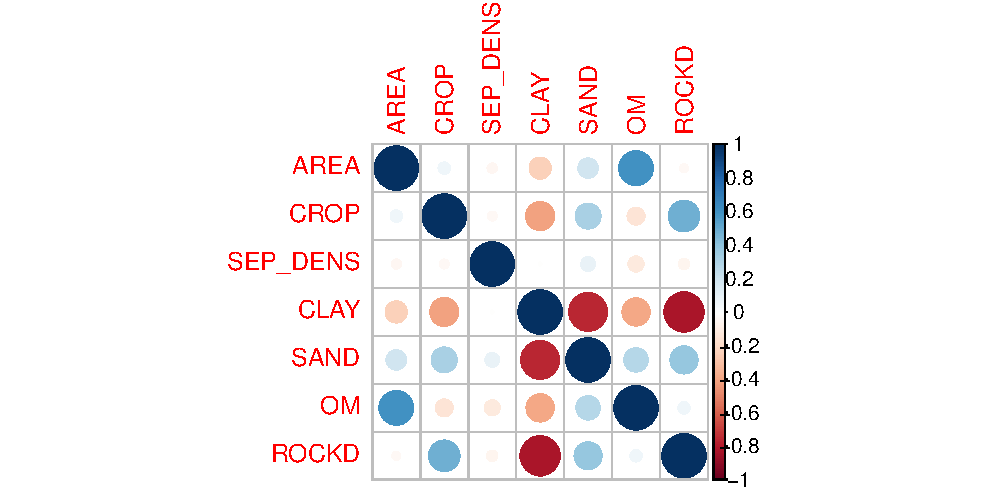
\includegraphics[width=0.6\textwidth]{./figures/corr.pdf}
	\caption{Plot of correlation structure}
	\label{fig: correlation}
\end{figure}

In summary, we choose landscape-based data as input data for our models. The data were quantified at the stream segment scale (1:100,000) defined by the vector-based, segment-level catchments within the NHDPlus hydrologic spatial dataset. Using this dataset has the advantage of being easy to obtain. With the development of space technology, it is also very cheap to collect these data. We have uploaded all datasets and codes to our GitHub repository.\footnote{\url{https://github.com/mnazaal/aalto-bda-project}}

\subsection{R setup}
The full R code can be found in \texttt{MVP.r}:
\begin{lstlisting}[language=R]
#import packages to be used
library(gridExtra)
library(qgraph)
library(coda)
library(rstan)
library(ggplot2)
library(loo)
library(posterior)

#set stan options for parallel processing of HMC chains
rstan_options(auto_write = TRUE)
options(mc.cores = parallel::detectCores())
\end{lstlisting}

\subsection{Data processing}
We standardize the three predictors, including drainage area ($\beta_{log(AREA}$), crop cover ($\beta_{CROP}$), and density of septic systems($\beta_{SEP}$). 
\begin{lstlisting}[language=R]
#Function to scale and center predictors based on Gelman et al. 2006
MyStd <- function(x){ (x-mean(x))/(sd(x)*2)} #apply(x,2,MyStd)

#Apply same standardization to variables used to predict to unsampled catchments
x_predict <-  as.matrix(cbind(MyStd(log(streamCat[,4])),
                              MyStd(streamCat[,16]),
                              MyStd(streamCat[,19])
))
\end{lstlisting}

For the response variable, we use the dataset from EFLMR, which can be found in \texttt{OEPA\_WATER\_2012.csv}, which includes locations of OEPA bioassessment sites ($N=83$) across the EFLMR watershed. 
\begin{lstlisting}[language=R]
#convert fish abundance to presence-absence (binary; 0 or 1)
y <- as.matrix(ifelse(modelData[,c(6:82,146)]>0,1,0))
\end{lstlisting}

\section{Description of models}
\label{sec: models}
In the section, we will introduce two models used in this report. They are: (1) Hierarchical model, and (2) Pooling model. 

\subsection{Hierarchical model}
Our hierarchical model is shown in Eq. (\ref{eq: hier}), and its illustration can be found in Figure \ref{fig: hier_model_illustration}. As introduced in Section \ref{description}, our objective is to predict the probability of the occurrence of total phosphorus (TP). The occurrence of TP can be determined by several factors. In this report, we have selected drainage area (AREA, $\beta_\text{AREA}$), crop cover (CROP, $\beta_\text{CROP}$), and density of septic systems (SEP, $\beta_\text{SEP}$) as our input features. The intercept is represented by $\beta_0$. 


\begin{align}
    &P(y_n=1) = \text{logit}^{-1} (\beta_0+\beta_n  X_n), \forall n=1,\cdots,N\\
    &\beta_{0} \sim N(\mu_0,\sigma_0)\\
    &\beta_{k} \sim N(\mu_1,\sigma_1)
    \label{gp_eq}
\end{align}

\begin{figure}[!ht]
	\centering
	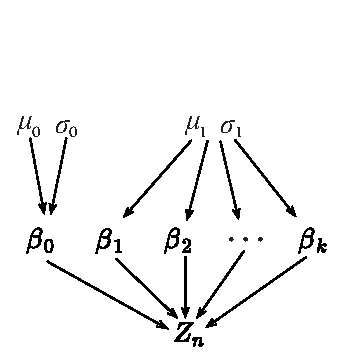
\includegraphics[width=0.3\textwidth]{./figures/hier_model.eps}
	\caption{Illustration of hierarchical model}
	\label{fig: hier_model_illustration}
\end{figure}

In the hierarchical model, the hyperparameter of $\beta_0$ are $\mu_0$ and $\sigma_0$. The prior of $\mu_0$ is a normal distribution with mean of 0 and standard deviation of 10, and $\sigma_0$ is subjected to a gamma distribution with $\alpha=1,\beta=1$. Like Gelman and Hill \cite{gelman2006data}, for the weights of the Bayesian linear regression model $\beta_{k}$. The weights also follow a normal distribution $N(\mu_1,\sigma_1)$, where ${\mu}_1$ is the hyperparameter for the mean values, and $\sigma_1$ is the hyperparameter for the standard deviation. ${\mu}_1$ is subjected to a normal distribution following mean value of 0 and standard deviation of 20. $X_n$ is the input matrix including all factors that can influence the occurrence of TP. 

\subsection{Gaussian Process model}

In this subsection, we consider presenting the linear model as a Gaussian process. Specifically, we extend the proposed hierarchical linear models to include nonlinear effects and implicit interactions. We describe the basic model as follows
\begin{align}
    &P(y_n=1) = \text{Bernoulli(logit} (f(X_n)), \forall n=1,\cdots,N. \label{gp}\\
    &f(X_n) \sim \text{GP(0, $\boldsymbol{K}$)} \label{gp_eq}
\end{align}
where the response y of TP has N sites by a receptor, representing the response of a receptor in the nth site. The response data is binary, which takes on the values 1 if the receptor is present and 0 if absent. The predictor variable matrix $X$ has $N$ sites as data size, and $K$ features or predictors. Therefore, in this project, we consider a multivariate regression problem in Gaussian process. 

Note that we use the exponentiated quadratic kernel to define the covariance between $f(X_i)$ and $f(X_i)$ where $f:\mathbb{R}^K\rightarrow \mathbb{R}$ is a function that we aim to model:

\begin{equation}\label{kernel}
    \text{cov}(f(X_i),f(X_i)) = k(X_i,X_j) = \alpha^2 \exp{\bigg(-\frac{1}{2\rho^2}\sum_{k=1}^{K}(X_{i,k}-X_{j,k})^2\bigg)}
\end{equation}
where $\alpha$ and $\rho$ are constrained to be positive. We use one variant of the exponentiated quadratic covariance function in Stan. Thus, the Gaussian process in \eqref{gp_eq} is based on a covariance matrix, $\boldsymbol{K} \in \mathbb{R}^{K\times K}$, where $\boldsymbol{K}_{i,j}=k(X_i,X_j)$, which is necessarily symmetric and positive semidefinite by construction. For simplicity, we use just one lengthscale in the exponentiated quadratic kernel for the three-dimensional model in \eqref{gp}.

In problem \eqref{gp}, we predict the ecological risk of water using logistic regression instead of analyzing the correlation between fishes and TP with the linear regression model. In \cite{martin2018empirically}, the author used $Z$ as a latent variable, in which the rows follow D-dimensional multivariate normal distributions, which are governed by a common correlation matrix $\Omega$. In our GP model, we do not consider the co-occurrence of stressors (i.e., TP) and receptors (fishes). 

\section{Weakly informative priors their choices} 
% Informative or weakly informative priors, and justification of their choices
\subsection{Priors of the hierarchical model}
In this report, for the hierarchical model, we utilized weakly informative priors. The justification of our choices are introduced below. 
\begin{itemize}
    \item For the intercept $\beta_0$, its hyperparameters are selected as  $\mu_0 \sim N(0,20)$. Since we have no idea of how will the mean value of the intercept will be. However, we can understand that it can be around zero if the weights are good. Thus, we select a normal distribution $N(0,20)$ as the prior for the mean value of the intercept. For the standard deviation, as it should be greater than zero, and  $\gamma(2,2)$ is employed. 
    \item For a weight of a factor, we assume that it is subjected to a normal distributions $N(\mu_1,\sigma_1)$. The prior of the mean values $\mu_1$ are set to be subjected to a normal distribution $N(0,30)$. Because there are several weights that are selected, we have increased the standard derivation from 20 to 30 compared to the intercept's mean value. For the standard derivation of the normal distribution $\sigma_1$, $\gamma(3,3)$ is selected as it should be greater than 0. The Gamma distribution can be found in Figure \ref{fig: gamma distribution}, where k = $\alpha$, and $\theta=1/\beta$ \cite{Gamma}. 
\end{itemize}

\begin{figure}[!ht]
	\centering
	\includegraphics[width=0.5\textwidth]{./figures/Gamma_distribution.eps}
	\caption{Gamma distribution}
	\label{fig: gamma distribution}
\end{figure}

\subsection{Priors of the Gaussian Process model}
In this our Gaussian process model, the hyperparameter comprises $\alpha$ and $\rho$ in \eqref{kernel}, for which we can construct appropriate priors. The justification of our choices are introduced below. 
\begin{itemize}
    \item For the Gaussian process \eqref{gp_eq}, it has prior with zero mean and exponentiated quadratic covariance function. In this project, we set zero mean for Gaussian process. It is on the one hand for an easier interpretation of the model, on the other hand for simplicity.
    \item In the exponentiated quadratic covariance function \eqref{kernel}, the hyperparameters controlling the covariance function of a Gaussian process can be fit by assigning them priors. In our second model, the priors on the parameters should be defined based on prior knowledge of the scale of the output values ($\alpha$) and the scale at which distances are measured among inputs ($\rho$).
\end{itemize}


\section{Stan codes}
% Stan, rstanarm or brms code (what options were used. This is also more clear as combination of textual explanation and the actual code line.)
\subsection*{Model 1: Hierarchical model}
We illustrate how to write Stan code that computes and stores the likelihood using the model example from Section \ref{sec: models}. We save the .stan code of model 1 in the file \texttt{Hier\_model\_TP.stan}. 
\begin{lstlisting}
data {
 int<lower=1> K;  //features dimension
 int<lower=1> D;
 int<lower=1> N1; //samples for training
 int<lower=1> N2; //samples for test
 int<lower=1> NN; //samples for prediction
 int idx1[N1]; //indices for training observations
 int idx2[N2]; //indices for test observations
 int<lower=1> M; //samples for marginal effects est
 int<lower=0,upper=1> y[N1+N2, D];
 int<lower=0,upper=1> Y[N1+N2];
 int trials[N1+N2];
 matrix[N1+N2,K]  x; //xxxxxx
 vector[K] X[NN];
 matrix[NN,K] x_predict;
 matrix[M,K] x_m_1; //marginal effect AREA
 matrix[M,K] x_m_2; //marginal effect CROP
 matrix[M,K] x_m_3; //marginal effect SEP
 }
parameters {
vector[N1+N2] beta0;
matrix[N1+N2,K] betak; //beta k
real mu_beta0;
real <lower=0> sigma_beta0;
vector[K] mu_betak;
real <lower=0> sigma_betak;
 }
transformed parameters{
 vector[N1+N2] f;
for (i in 1:(N1+N2)){
 f[i] = betak[i,] * x[i,]' + beta0[i];
}
}
model {
  // priors
  mu_beta0 ~ normal(0, 10);
  sigma_beta0 ~ gamma(1, 1);
  beta0 ~ normal(mu_beta0, sigma_beta0);
  for (i in 1:K){
  mu_betak[i] ~ normal(0, 20);
  }
  
  sigma_betak ~ gamma(2, 2);
  
 for (i in 1:K)
  betak[,i] ~ normal(mu_betak[i], sigma_betak);
//likelihood
 Y[idx1] ~ binomial_logit(trials[idx1], f[idx1]);
 }    
generated quantities{
 vector[N1] y_predict;
 vector[N1] f_invlogit;
 vector[N1] log_lik;
 // vector[NN] log_y_predict;
 // vector[N] y_new;
 vector[N2] log_y_new;
 
 for(i in 1:(N1)){
  y_predict[i] = binomial_rng(1, inv_logit(f[i]));
  f_invlogit[i] = inv_logit(f[i]);  //bernoulli_logit_rng(f[i])
  log_lik[i] = bernoulli_logit_lpmf(Y[i] | inv_logit(f[i]));
 }
 
 for(i in 1:N2){
  log_y_new[i] = binomial_logit_lpmf(Y[idx2[i]] | trials[idx2[i]], f[idx2[i]]);
 }
 
}
\end{lstlisting}

\subsection*{Model 2: Gaussian process}

The .stan code of model 2 is in the file \texttt{GP.stan}.

\begin{lstlisting}
functions {
	//GP covariance function
	vector gp(vector[] x, real sdgp, real lscale, vector zgp) { 
		matrix[size(x), size(x)] cov;
		cov = cov_exp_quad(x, sdgp, lscale);
		for (n in 1:size(x)) {
			cov[n, n] = cov[n, n] + 1e-12;
		}
		return cholesky_decompose(cov) * zgp;
	}
}
data {
 int<lower=1> K;  //features dimension
 int<lower=1> D;
 int<lower=1> N1; //samples for training
 int<lower=1> N2; //samples for test
 int<lower=1> NN; //samples for prediction
 int idx1[N1]; //indices for training observations
 int idx2[N2]; //indices for test observations
 int<lower=1> M; //samples for marginal effects est
 int<lower=0,upper=1> y[N1+N2, D];
 int<lower=0,upper=1> Y[N1+N2];
 int trials[N1+N2];
 vector[K] x[N1+N2];
 vector[K] X[NN];
 matrix[NN,K] x_predict;
 matrix[M,K] x_m_1; //marginal effect AREA
 matrix[M,K] x_m_2; //marginal effect CROP
 matrix[M,K] x_m_3; //marginal effect SEP
 }
parameters {
 real<lower=0> alpha[K]; // lengthscale of f
 real<lower=0> rho[K];       // scale of f
 matrix[N1+N2,K] eta;
 }
transformed parameters{
	vector[N1+N2] f;
	
	f = gp(x, alpha[1], rho[1], eta[,1]);

}
model {
  // priors
 alpha ~ normal(0, 1);
 rho ~ normal(0, 1);
 to_vector(eta) ~ normal(0,1);
 Y[idx1] ~ binomial_logit(trials[idx1], f[idx1]);
 }    
generated quantities{
	vector[N1] y_predict;
	vector[N1] f_invlogit;
	vector[N1] log_lik;
	// vector[NN] log_y_predict;
	// vector[N] y_new;
	vector[N2] log_y_new;
	
	for(i in 1:(N1)){
		y_predict[i] = binomial_rng(1, inv_logit(f[i]));
		f_invlogit[i] = inv_logit(f[i]);  //bernoulli_logit_rng(f[i])
		log_lik[i] = bernoulli_logit_lpmf(Y[i] | inv_logit(f[i]));
	}
	
	for(i in 1:N2){
		log_y_new[i] = binomial_logit_lpmf(Y[idx2[i]] | trials[idx2[i]], f[idx2[i]]);
	}
	
}

\end{lstlisting}

\section{How the Stan model was run}
% How the Stan model was run, that is, what options were used. This is also more clear as combination of textual explanation and the actual code line.
\subsection*{Model 1: Hierarchical model}
In the following line, we used Rstan to compile our model. The working environment is: 
\begin{itemize}
\item Operate system: Ubuntu 22.04.1 LTS
\item Processor: i7-9750 H CPU @ 2.60 GHz $\times$ 8
\item Memory: 7.7 GiB
\end{itemize}
\begin{lstlisting}[language=R]
HierfitDSO <- stan_model(file = "models/Hier_model_TP.stan") # Here Rstan used to compile our model
\end{lstlisting}

Then, the used data are put into a list that is convenient to be used for later fit. 

\begin{lstlisting}[language=R]
HierdataList <- list(
y=y,
Y=Y,
x=x, 
X=x_predict,
x_m_1=as.matrix(cbind(seq(min(x[,1]),max(x[,1]),length.out=M),rep(0, M), rep(0, M))),
x_m_2=as.matrix(cbind(rep(0, M), seq(min(x[,2]),max(x[,2]),length.out=M), rep(0, M))),
x_m_3=as.matrix(cbind(rep(0, M), rep(0, M), seq(min(x[,3]),max(x[,3]),length.out=M))),
K=ncol(x), 
D=ncol(y), 
N1=N1,
N2=N2,
NN=NN,
M=M,
idx1=idx1,
idx2=idx2,
trials=trials,
x_data=x,
x_predict=x_predict) # predictive data
\end{lstlisting}

Finally, we fitted the model using the above data. The optional are introduced below. 

\begin{itemize}
\item The number of chains: 4
\item The number of interation: 10000
\item The number of cores: 4
\item The period for saving samples: 1
\item Initial values specification: 0
\item max\_treedepth: 15, as there are warnings indicating that 10 is not enough for fitting this model.  
\end{itemize}

\begin{lstlisting}[language=R]
Hierfit <- sampling(object=HierfitDSO,
data=HierdataList,
chains=4, # the number of chains we used
iter=15000, # the number of interation we used
cores=4, # the number of cores we used
thin=1, # the period for saving samples is set to 1
init=0, # Initial values specification
control = list( # we added several options to improve sampling
adapt_delta=0.98, # adapt_delta default=0.8
max_treedepth =15) # max_treedepth default= 10
\end{lstlisting}

\subsection*{Model 2: GP model}
In the following line, we used Rstan to compile our model. The working environment is: 
\begin{itemize}
\item Operate system: Windows 10
\item Processor: i5-1135G7 CPU @ 2.40 GHz $\times$ 6
\item Memory: 16 GiB
\end{itemize}

\begin{lstlisting}[language=R]
GPfitDSO <- stan_model(file = "models/GP.stan") # Here Rstan used to compile our model
\end{lstlisting}

Then, the used data are put into a list that is convenient to be used for fit of the GP model. 

\begin{lstlisting}[language=R]
GPdataList <- list(y=y,
Y=Y,
x=x, 
X=x_predict,
x_m_1=as.matrix(cbind(seq(min(x[,1]),max(x[,1]),length.out=M),rep(0, M), rep(0, M))),
x_m_2=as.matrix(cbind(rep(0, M), seq(min(x[,2]),max(x[,2]),length.out=M), rep(0, M))),
x_m_3=as.matrix(cbind(rep(0, M), rep(0, M), seq(min(x[,3]),max(x[,3]),length.out=M))),
K=ncol(x), 
D=ncol(y), 
N1=N1,
N2=N2,
NN=NN,
M=M,
idx1=idx1,
idx2=idx2,
trials=trials,
x_data=x,
x_predict=x_predict)#real data 
\end{lstlisting}

Finally, we fitted the model using the above data. The optional are introduced below. 

\begin{itemize}
\item The number of chains: 4
\item The number of interation: 1000
\item The number of cores: 4
\item The period for saving samples: 1
\item Initial values specification: 0
\item max\_treedepth: 15, as there are warnings indicating that 10 is not enough for fitting this model.  
\end{itemize}

\begin{lstlisting}[language=R]
GPfit <- sampling(object=GPfitDSO,
data=GPdataList,
chains=4,
iter=1000,
cores=4,
thin=1,
init=0,
control = list( #add options to improve sampling (divergent transitions)
adapt_delta=0.98, #default=0.8
max_treedepth =15 #default= 10
)
)
\end{lstlisting}

\section{Convergence diagnostics}
% Convergence diagnostics, $\hat{R}$, ESS, divergences, what was done if it did not work the first time etc.
\subsection*{Model 1: Hierarchical model}
For the hierarchical model, at first when we have only 1000 iterations, we found that the $\hat{R}$ for our hyperparameter is a little bit high, which means that our MCMC progress may not converge well. Therefore, we improved the iterations to 15000, then all $\hat{R}$ values are smaller than 1.05, meaning that the MCMC for all posterior values converge now.  

But we found that our hierarchical model, the Bulk Effective Samples Size (ESS) value is relatively low, which means that the posterior means and medians may not be quite reliable. We will find more ways to solve this problem. The interesting thing is that when we did not use the hierarchical model, instead, we used the separate model, this problem did not emerge. We would like to have some discussions with the reviewers and TAs after the presentation. In Table \ref{hier_results}, the first 10 lines of the posterior are shown, and the full lines can be found in our github website \footnote{\url{https://github.com/mnazaal/aalto-bda-project/blob/main/report/Hier_model_TP.txt}}. 

Inference for Stan model: \texttt{Hier\_model\_TP.stan}:

4 chains, each with iter=1000; warmup=500; thin=1; 

post-warmup draws per chain=500, total post-warmup draws=2000.


\begin{table}[!ht]
\centering
\caption{Results of fitting: first 10 lines$^1$}
\label{hier_results}
\begin{tabular}{lllllllllll}
\hline
              & mean & se\_mean & sd   & 2.50\% & 25\% & 50\% & 75\% & 97.50\% & n\_eff & Rhat \\ \hline
beta0{[}1{]}  & 1.51 & 0.02     & 1.97 & -2.64  & 0.53 & 1.47 & 2.51 & 5.64    & 7893   & 1    \\
beta0{[}2{]}  & 2.64 & 0.08     & 2.22 & -0.48  & 1.24 & 2.12 & 3.56 & 8.3     & 774    & 1    \\
beta0{[}3{]}  & 0.72 & 0.03     & 1.78 & -3.56  & -0.1 & 0.96 & 1.76 & 3.78    & 3726   & 1    \\
beta0{[}4{]}  & 3.64 & 0.16     & 2.62 & 0.33   & 1.76 & 2.99 & 4.91 & 10.34   & 280    & 1.01 \\
beta0{[}5{]}  & 2.72 & 0.09     & 2.28 & -0.41  & 1.29 & 2.2  & 3.65 & 8.57    & 615    & 1.01 \\
beta0{[}6{]}  & 2.8  & 0.1      & 2.31 & -0.36  & 1.34 & 2.26 & 3.76 & 8.64    & 584    & 1.01 \\
beta0{[}7{]}  & 2.14 & 0.05     & 2.49 & -2.32  & 0.83 & 1.81 & 3.17 & 8.11    & 2154   & 1    \\
beta0{[}8{]}  & 3.01 & 0.11     & 2.39 & -0.22  & 1.43 & 2.42 & 4.07 & 9.14    & 463    & 1.01 \\
beta0{[}9{]}  & 3.96 & 0.17     & 2.78 & 0.49   & 1.91 & 3.28 & 5.37 & 10.98   & 257    & 1.01 \\
beta0{[}10{]} & 1.07 & 0.02     & 1.84 & -3.15  & 0.21 & 1.2  & 2.07 & 4.57    & 11777  & 1    \\ \hline
\end{tabular}
\end{table}


\subsection{GP model}


\begin{table}[!ht]
\centering
\caption{Results of fitting: first 10 lines$^1$}
\label{gp_results}
\begin{tabular}{lllllllllll}
\hline
             & mean  & se\_mean & sd   & 2.50\% & 25\%  & 50\%  & 75\% & 97.50\% & n\_eff & Rhat \\ \hline
alpha{[}1{]} & 1.25  & 0.01     & 0.48 & 0.43   & 0.91  & 1.2   & 1.55 & 2.31    & 1379   & 1    \\
alpha{[}2{]} & 0.8   & 0.01     & 0.62 & 0.03   & 0.31  & 0.66  & 1.14 & 2.29    & 4055   & 1    \\
alpha{[}3{]} & 0.8   & 0.01     & 0.59 & 0.03   & 0.32  & 0.71  & 1.13 & 2.24    & 2414   & 1    \\
rho{[}1{]}   & 1.06  & 0.01     & 0.48 & 0.41   & 0.71  & 0.96  & 1.33 & 2.21    & 1024   & 1    \\
rho{[}2{]}   & 0.78  & 0.01     & 0.61 & 0.03   & 0.3   & 0.64  & 1.15 & 2.29    & 2674   & 1    \\
rho{[}3{]}   & 0.81  & 0.01     & 0.58 & 0.04   & 0.34  & 0.69  & 1.16 & 2.18    & 2042   & 1    \\
sigma        & 4.09  & 0.06     & 3.18 & 0.13   & 1.53  & 3.46  & 5.87 & 11.67   & 3055   & 1    \\
eta{[}1,1{]} & -0.2  & 0.01     & 0.55 & -1.28  & -0.54 & -0.2  & 0.12 & 0.91    & 1390   & 1    \\
eta{[}1,2{]} & -0.01 & 0.02     & 0.99 & -1.88  & -0.67 & -0.02 & 0.68 & 1.93    & 3173   & 1    \\
eta{[}1,3{]} & 0     & 0.02     & 0.97 & -1.96  & -0.64 & 0.01  & 0.65 & 1.92    & 3117   & 1    \\ \hline
\end{tabular}
\end{table}


\section{Possible improvement}

% Posterior predictive checks and what was done to improve the model
here we will speak something about possible improvements. 

\begin{itemize}
\item more fishes 
\item Consider mode factors
\item ...
\end{itemize}


\section{Predictive performance assessment if applicable}

% \begin{table}[!ht]
% \centering
% \caption{loo validation}
% \label{loo_val}
% \begin{tabular}{@{}lll|lll@{}}
% \toprule
% \multicolumn{3}{l|}{Hierarchical model} & \multicolumn{3}{l}{GP   model} \\ \midrule
%                & Estimate     & SE      &             & Estimate  & SE   \\
% elpd\_loo      & -36.5        & 2.4     & elpd\_loo   & -38.6     & 2.5  \\
% p\_loo         & 0.6          & 0.1     & p\_loo      & 0.2       & 0    \\
% looic          & 73           & 4.9     & looic       & 77.2      & 5    \\ \bottomrule
% \end{tabular}
% \end{table}

\begin{figure}[!h]
\centering
\subfigure[Hier model]{
    \begin{minipage}[t]{0.5\linewidth}
        \centering
        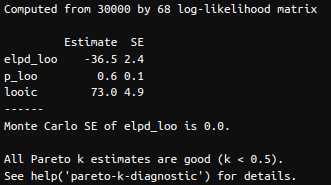
\includegraphics[width=0.835\textwidth]{./figures/loo1.png}
    \end{minipage}%
}%
\subfigure[GP model]{
    \begin{minipage}[t]{0.5\linewidth}
        \centering
        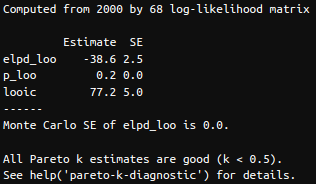
\includegraphics[width=0.8\textwidth]{./figures/loo2.png}
    \end{minipage}%
}%
\caption{hier}
\label{fig: hier results}
\end{figure}

% Computed from 30000 by 68 log-likelihood matrix
%          Estimate  SE
% elpd_loo    -36.5 2.4
% p_loo         0.6 0.1
% looic        73.0 4.9
% ------
% Monte Carlo SE of elpd_loo is 0.0.

% All Pareto k estimates are good (k < 0.5).
% See help('pareto-k-diagnostic') for details.


% Computed from 2000 by 68 log-likelihood matrix

%          Estimate  SE
% elpd_loo    -38.6 2.5
% p_loo         0.2 0.0
% looic        77.2 5.0
% ------
% Monte Carlo SE of elpd_loo is 0.0.

% All Pareto k estimates are good (k < 0.5).
% See help('pareto-k-diagnostic') for details.

In Figure , there are 27 species and the total phosphorus (represented by P\_exc in red) are investigated.

% \begin{figure}[!h]
% \centering
% \subfigure[Intercept]{
%     \begin{minipage}[t]{0.5\linewidth}
%         \centering
%         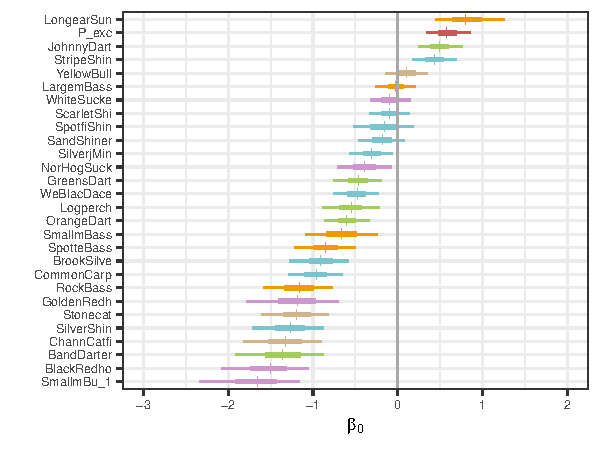
\includegraphics[width=1.0\textwidth]{./figures/intercept_plot.pdf}
%     \end{minipage}%
% }%
% \subfigure[AREA]{
%     \begin{minipage}[t]{0.5\linewidth}
%         \centering
%         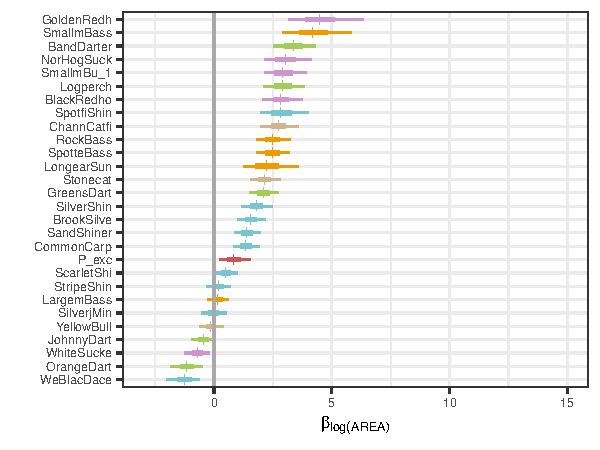
\includegraphics[width=1.0\textwidth]{./figures/area_plot.pdf}
%     \end{minipage}%
% }%

% \subfigure[CROP]{
%     \begin{minipage}[t]{0.5\linewidth}
%         \centering
%         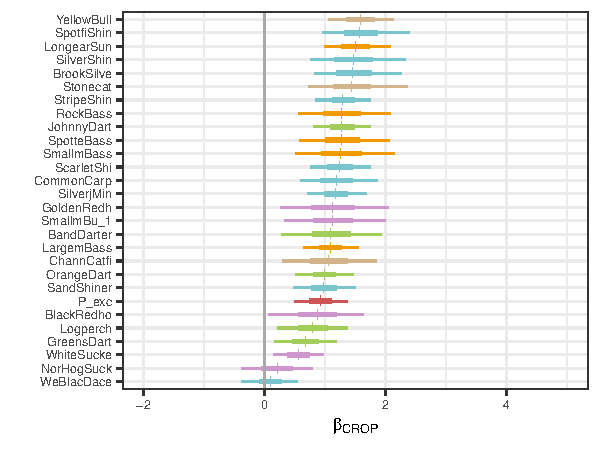
\includegraphics[width=1.0\textwidth]{./figures/crop_plot.pdf}
%     \end{minipage}%
% }%
% \subfigure[SEP]{
%     \begin{minipage}[t]{0.5\linewidth}
%         \centering
%         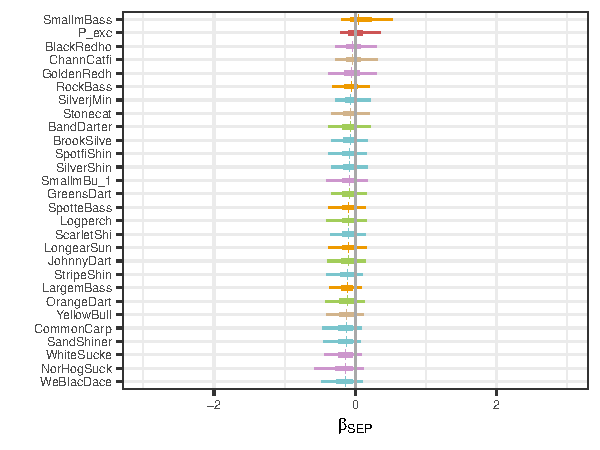
\includegraphics[width=1.0\textwidth]{./figures/sep_plot.pdf}
%     \end{minipage}%
% }%
% \caption{hier}
% \label{fig: hier results}
% \end{figure}


\section{Sensitivity analysis with respect to prior choices}
In this section, we can select more priors and show different results using different priors. 

\section{Discussion of issues and potential improvements}

In this section, we will discuss about issues and improvements. 

(1) more iteration problem 

(2) Prior selection

\section{Conclusion}
% what was learned from the data analysis

\section{Self-reflection of what the group learned while making the project}

\begin{itemize}
\item A good dataset
\item Find partners
\end{itemize}
   


\begin{spacing}{1.5} 
\bibliography{Ref.bib}
\end{spacing}


\end{document}
